\documentclass{beamer}
\usepackage{amsmath}
\usepackage[english]{babel} %set language; note: after changing this, you need to delete all auxiliary files to recompile
\usepackage[utf8]{inputenc} %define file encoding; latin1 is the other often used option
\usepackage{csquotes} % provides context sensitive quotation facilities
\usepackage{graphicx} %allows for inserting figures
\usepackage{booktabs} % for table formatting without vertical lines
\usepackage{textcomp} % allow for example using the Euro sign with \texteuro
\usepackage{stackengine}
\usepackage{wasysym}
\usepackage{tikzsymbols}
\usepackage{textcomp}
% ELIMINAR COMANDOS DE NAVEGACION%%%%%%%%%%%
\setbeamertemplate{navigation symbols}

%\newcommand{\bubblethis}[2]{
 %       \tikz[remember picture,baseline]{\node[anchor=base,inner sep=0,outer sep=0]%
 %       (#1) {\underline{#1}};\node[overlay,cloud callout,callout relative pointer={(0.2cm,-0.7cm)},%
 %       aspect=2.5,fill=yellow!90] at ($(#1.north)+(-0.5cm,1.6cm)$) {#2};}%
 %   }%
%\tikzset{face/.style={shape=circle,minimum size=4ex,shading=radial,outer sep=0pt,
 %       inner color=white!50!yellow,outer color= yellow!70!orange}}

%% Some commands to make the code easier
\newcommand{\emoticon}[1][]{%
  \node[face,#1] (emoticon) {};
  %% The eyes are fixed.
  \draw[fill=white] (-1ex,0ex) ..controls (-0.5ex,0.2ex)and(0.5ex,0.2ex)..
        (1ex,0.0ex) ..controls ( 1.5ex,1.5ex)and( 0.2ex,1.7ex)..
        (0ex,0.4ex) ..controls (-0.2ex,1.7ex)and(-1.5ex,1.5ex)..
        (-1ex,0ex)--cycle;}
\newcommand{\pupils}{
  %% standard pupils
  \fill[shift={(0.5ex,0.5ex)},rotate=80] 
       (0,0) ellipse (0.3ex and 0.15ex);
  \fill[shift={(-0.5ex,0.5ex)},rotate=100] 
       (0,0) ellipse (0.3ex and 0.15ex);}

\newcommand{\emoticonname}[1]{
  \node[below=1ex of emoticon,font=\footnotesize,
        minimum width=4cm]{#1};}
\usepackage{scalerel}
\usetikzlibrary{positioning}
\usepackage{xcolor,amssymb}
\newcommand\dangersignb[1][2ex]{%
  \scaleto{\stackengine{0.3pt}{\scalebox{1.1}[.9]{%
  \color{red}$\blacktriangle$}}{\tiny\bfseries !}{O}{c}{F}{F}{L}}{#1}%
}
\newcommand\dangersignw[1][2ex]{%
  \scaleto{\stackengine{0.3pt}{\scalebox{1.1}[.9]{%
  \color{red}$\blacktriangle$}}{\color{white}\tiny\bfseries !}{O}{c}{F}{F}{L}}{#1}%
}
\usepackage{fontawesome} % Social Icons
\usepackage{epstopdf} % allow embedding eps-figures
\usepackage{tikz} % allows drawing figures
\usepackage{amsmath,amssymb,amsthm} %advanced math facilities
\usepackage{lmodern} %uses font that support italic and bold at the same time
\usepackage{hyperref}
\usepackage{tikz}
\usepackage{tcolorbox}

\usefonttheme[onlymath]{serif} %set math font to serif ones

\definecolor{beamerblue}{rgb}{0.2,0.2,0.7} %define beamerblue color for later use

%%% defines highlight command to set text blue
\newcommand{\highlight}[1]{{\color{blue}{#1}}}


%%%%%%% commands defining backup slides so that frame numbering is correct

\newcommand{\backupbegin}{
   \newcounter{framenumberappendix}
   \setcounter{framenumberappendix}{\value{framenumber}}
}
\newcommand{\backupend}{
   \addtocounter{framenumberappendix}{-\value{framenumber}}
   \addtocounter{framenumber}{\value{framenumberappendix}}
}

%%%% end of defining backup slides

%Specify figure caption, see also http://tex.stackexchange.com/questions/155738/caption-package-not-working-with-beamer
\setbeamertemplate{caption}{\insertcaption} %redefines caption to remove label "Figure".
%\setbeamerfont{caption}{size=\scriptsize,shape=\itshape,series=\bfseries} %sets figure  caption bold and italic and makes it smaller


\newtcolorbox{boxA}{
    fontupper = \bf,
    boxrule = 1.5pt,
    colframe = black % frame color
}

\usetheme{Boadilla}


% --------------------
% Overall information
% --------------------
\title[Economía I]{Economía I \vspace{4mm}
\\ Magistral 12: Competencia Perfecta}
\date{}
\author[Riottini]{Riottini Franco}
\vspace{0.4cm}
\institute[]{Universidad de San Andrés}  

\begin{document}

\begin{frame}
\titlepage
\centering

\includegraphics[scale=0.2]{../Figures/logoUDESA.jpg} 
\end{frame}


\begin{frame}
\frametitle{¿Se acuerdan del equilibrio de mercado?}
\centering
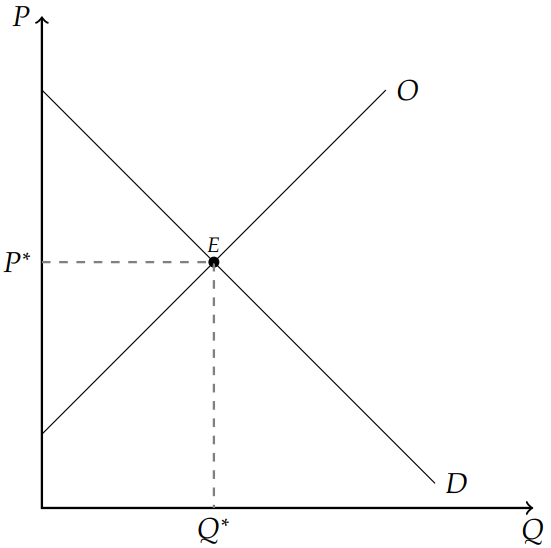
\includegraphics[scale=0.6]{../Figures/C21.1.png}
\end{frame}

\begin{frame}
\frametitle{Equilibrio}
\begin{itemize}
    \item En el precio de equilibrio, la oferta iguala a la demanda y el mercado se \textbf{vacia}.
    \item En el equilibrio, el excedente del consumidor y del productor es máximo y se producen todas las transacciones en las cuales la valoración por el bien es mayor que el costo de producirlo.
    \item Otros precios no son un equilibrio de Nash y tampoco son Pareto eficiente.
    \begin{itemize}
        \item Si $p > p^{*}$, entonces habría exceso de oferta.
        \item Si $p < p^{*}$, entonces habría exceso de demanda.
        \item Se asume que los productos son idénticos, por lo que los compradores estarían dispuestos a comprar a cualquier vendedor.
    \end{itemize}
\end{itemize}
\end{frame}

\begin{frame}{Tipos de mercado}
    ¿Que tipo de mercado vamos a estudiar?
    \begin{enumerate}
        \item Competencia perfecta: Gran cantidad de compradores y vendedores. Productos \textbf{homogéneos}.
        \item Competencia Monopolistica: Hay muchos compradores
        y vendedores que se caracterizan por ofrecer productos \textbf{heterogéneos}, es decir, de diferente
        calidad o características.
        \item Oligopolio: Muchos compradores pero pocos vendedores.
        \item Monopolio: Muchos compradores pero un solo productor.
    \end{enumerate}
\end{frame}

\begin{frame}
\frametitle{Competencia y empresas tomadoras de precios}
\begin{itemize}
    \item ¿Cuándo tenemos una mercado competitivo?
    \begin{enumerate}
        \item Muchos compradores y vendedores no diferenciados que actúan en forma independiente.
        \item El precio viene determinado por el mercado.
        \item Productos ofrecidos básicamente idénticos.
        \item Información perfecta de los consumidores y las empresas.
        \item Las firmas entran o salen del mercado libremente.
    \end{enumerate}
    \item En un mercado competitivo las firmas y los consumidores son tomadores de precios.
    \begin{itemize}
        \item Para la firma esto quiere decir que el precio de mercado es igual al ingreso marginal.
        \[ p = IMg = IMe \]
    \end{itemize}
\end{itemize}
\end{frame}

\begin{frame}{Precios determinados por el mercado}
    \begin{itemize}
        \item Las firmas son tomadoras de precios, eso quiere decir que no pueden:
        \begin{itemize}
            \item Influir en el precio de mercado.
            \item Beneficiarse de la elección de un precio diferente del precio de mercado.
        \end{itemize}
        \item La curva de demanda de estas firmas se vuelve plana.
        \item ¿Y la oferta de la firma?
        \end{itemize}
        \begin{boxA}
            \centering
            La empresa elige cantidad, no precio
        \end{boxA}
        \centering
        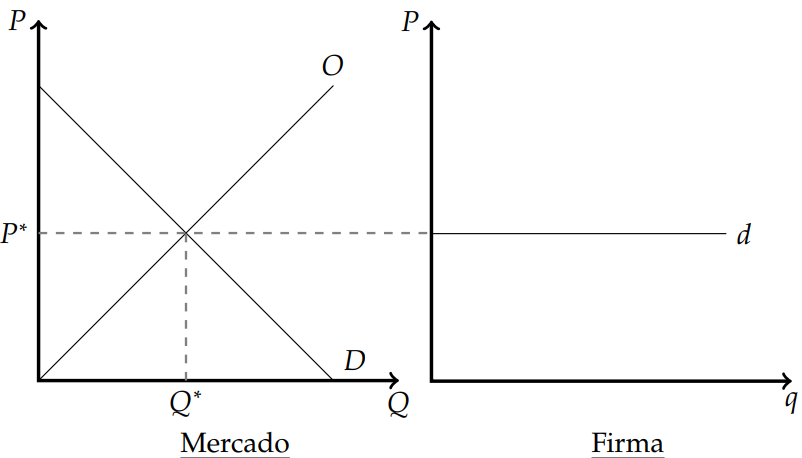
\includegraphics[scale=0.4]{../Figures/C21.2.png}
\end{frame}

\begin{frame}{El mercado de Chicago}
    \centering
    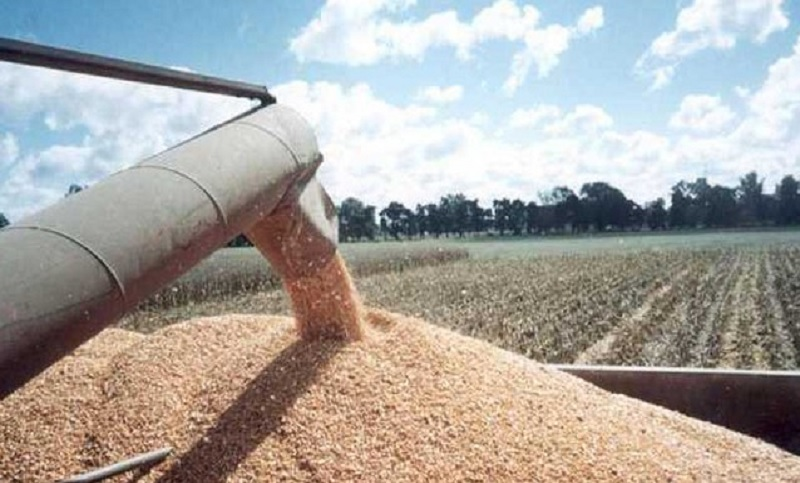
\includegraphics[scale=0.4]{../Figures/Mercado_Granos.jpg}
\end{frame}

\begin{frame}
\frametitle{¿Qué pasa en la empresa?}
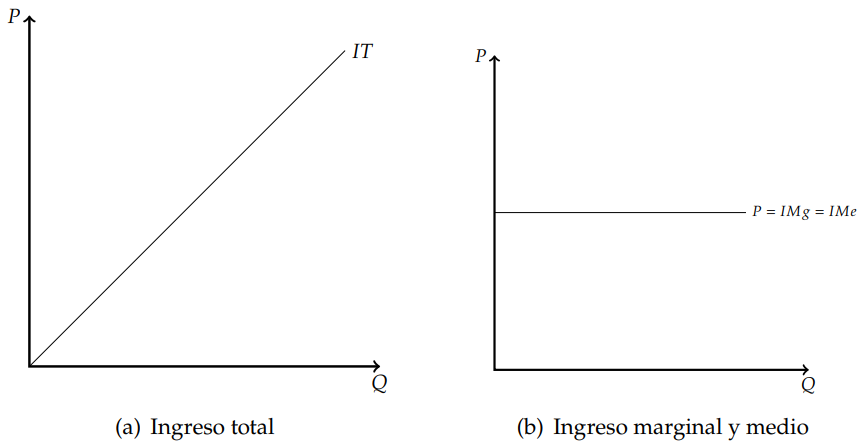
\includegraphics[scale=0.6]{../Figures/C21.4.png}
\end{frame}

\begin{frame}
    \frametitle{¿Qué pasa en la empresa?}
    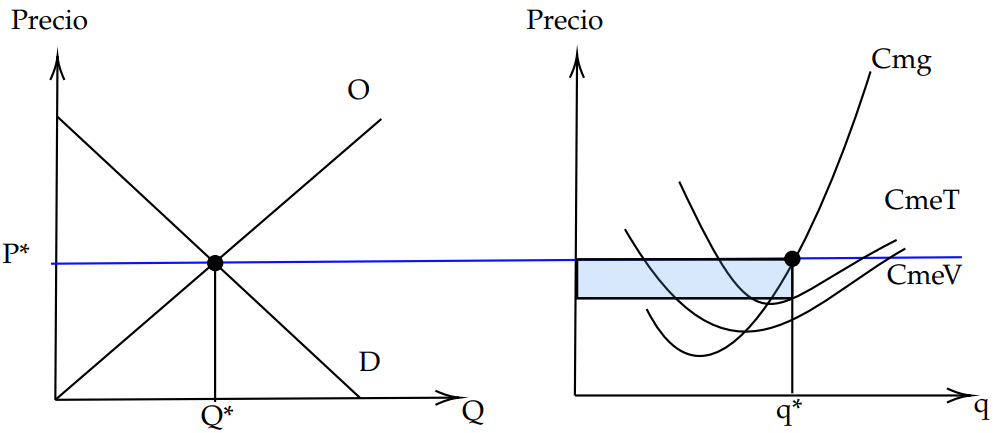
\includegraphics[scale=0.55]{../Figures/C21.5.png}
\end{frame}

\begin{frame}
\frametitle{¿Qué pasa si el precio es mayor que el costo marginal?}
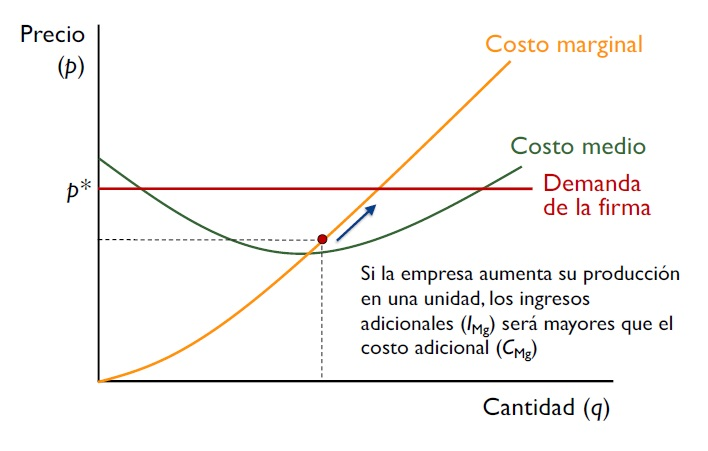
\includegraphics[scale=0.55]{../Figures/Tema_07.8_compperfecta2.jpg}
\end{frame}

\begin{frame}
\frametitle{¿Qué pasa si el precio es menor que el costo marginal?}
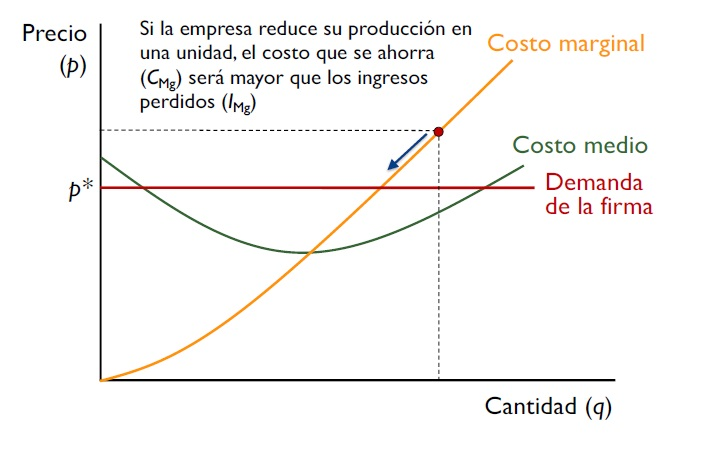
\includegraphics[scale=0.55]{../Figures/Tema_07.9_compperfecta3.jpg}
\end{frame}

\begin{frame}
\frametitle{La empresa maximiza beneficios, ¿cómo?}
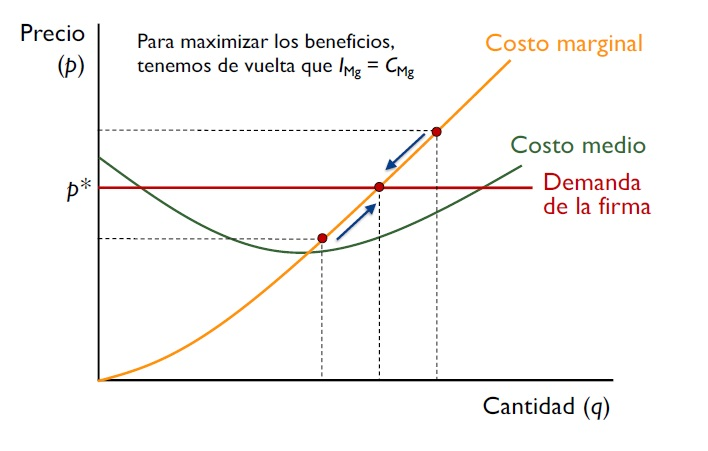
\includegraphics[scale=0.55]{../Figures/Tema_07.10_compperfecta4.jpg}
\end{frame}

\begin{frame}
\frametitle{Veamos un ejemplo}
\begin{itemize}
    \item Precio: \$32
    \item Costo marginal = $2Q^{2}$
\end{itemize}
\centering
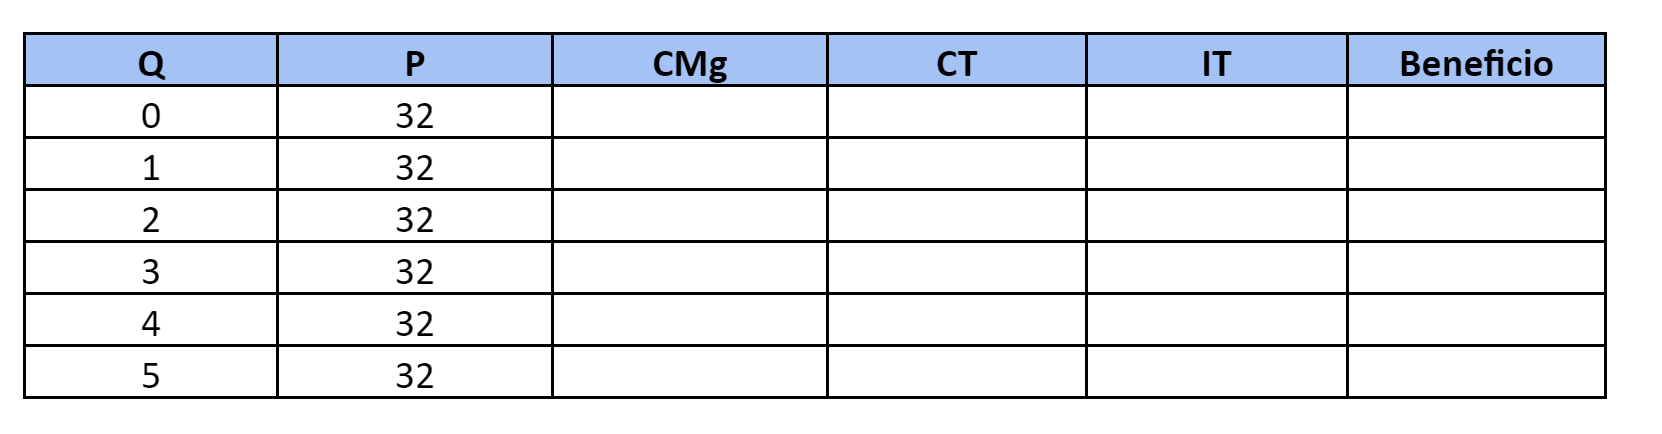
\includegraphics[scale=0.7]{../Figures/Ejemplo Competencia Perfecta.png}
\end{frame}

\begin{frame}
\frametitle{¿Habrá beneficio en este punto? SI!}
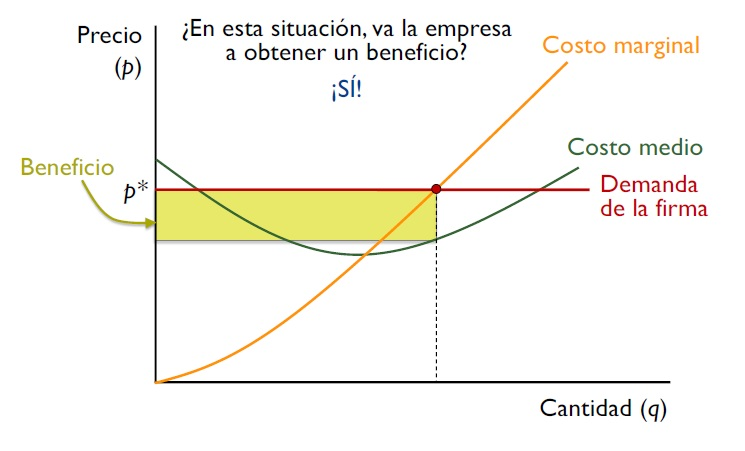
\includegraphics[scale=0.55]{../Figures/Tema_07.11_compperfecta5.jpg}
\end{frame}

\begin{frame}
\frametitle{¿Habrá beneficio en este punto? NO! ¿Hay perdida? SI!}
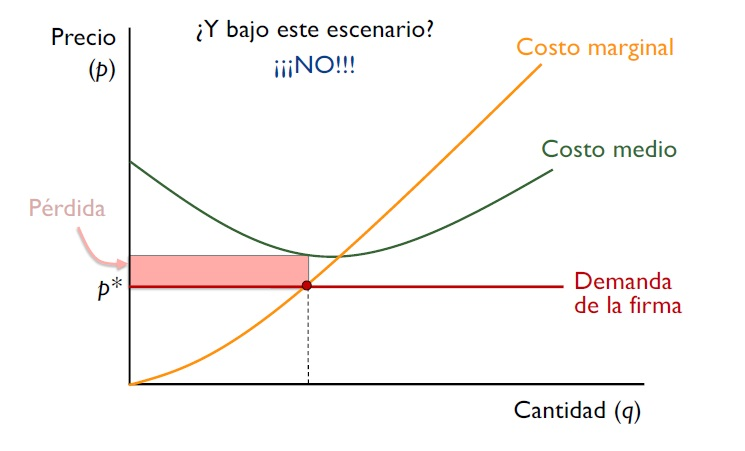
\includegraphics[scale=0.55]{../Figures/Tema_07.12_compperfecta6.jpg}
\end{frame}

\begin{frame}
\frametitle{¿Habrá beneficio extraordinario en este punto? NO! ¿Hay perdida? NO!}
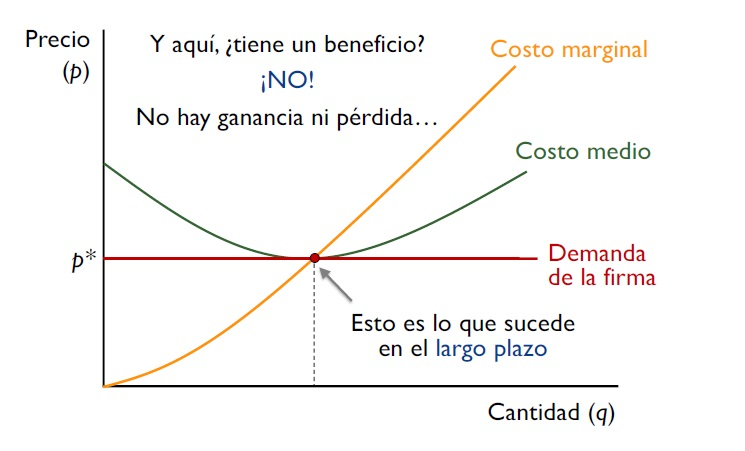
\includegraphics[scale=0.55]{../Figures/Tema_07.13_compperfecta7.jpg}
\end{frame}

\begin{frame}
    \frametitle{En el corto plazo}
    \begin{boxA}
        \centering
        En competencia perfecta, la empresa maximiza sus beneficios en el
        corto plazo cuando el ingreso marginal se iguala al costo marginal.
        Es decir, cuando el precio se iguala al costo marginal.
    \end{boxA}
    \begin{boxA}
        \centering
        En competencia perfecta, la empresa produce una cantidad positiva si el precio que observa en el mercado iguala o supera el costo
        medio variable en el punto donde maximiza sus beneficios.
    \end{boxA}

\end{frame}


\begin{frame}
\frametitle{¿Y en el largo plazo...}
\begin{itemize}
    \item Siempre que existan potenciales rentas (beneficios extraordinarios), va a haber firmas interesadas en entrar al mercado.
    \item Si los costos de entrada no son demasiado altos, estas firmas potenciales van a entrar.
    \item Al ingresar, las firmas van a presionar hacia abajo el precio de equilibrio, eliminando del mercado a las firmas menos eficientes.
    \item Los beneficios que atraen a potenciales entrantes comienzan a disiparse.
    \item En el largo plazo, estos beneficios van a desaparecer, serán iguales a 0.
    \end{itemize}
\end{frame}

\begin{frame}{¿Y en el largo plazo...}
    \begin{center}
    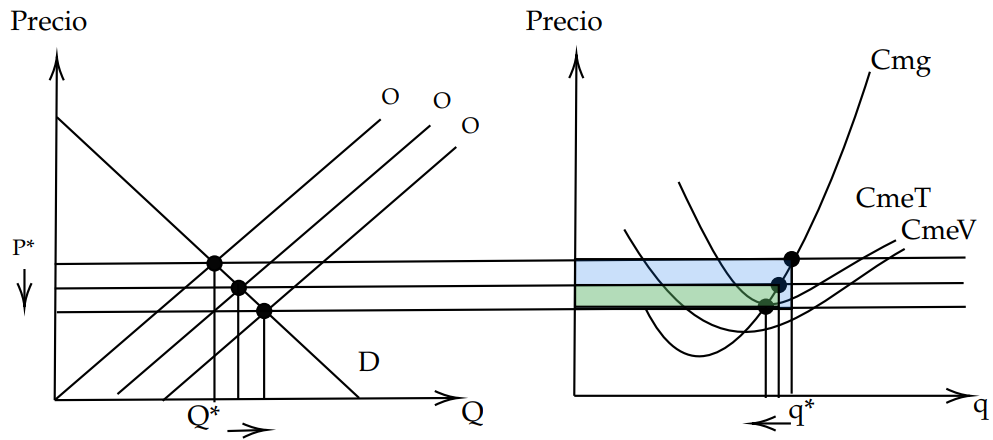
\includegraphics[scale=0.55]{../Figures/C21.6.png}
    \end{center}
\end{frame}

\begin{frame}
    \frametitle{¿Y en el largo plazo...}
    \begin{center}
    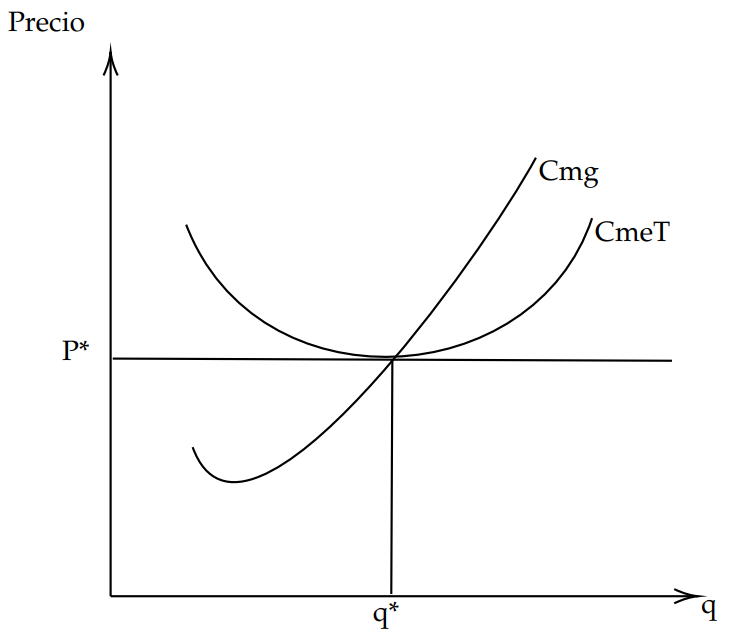
\includegraphics[scale=0.6]{../Figures/C21.7.png}
    \end{center}
\end{frame}

\begin{frame}
\frametitle{Recordemos lo que sucede en equilibrio... beneficios para todos!}
\begin{center}
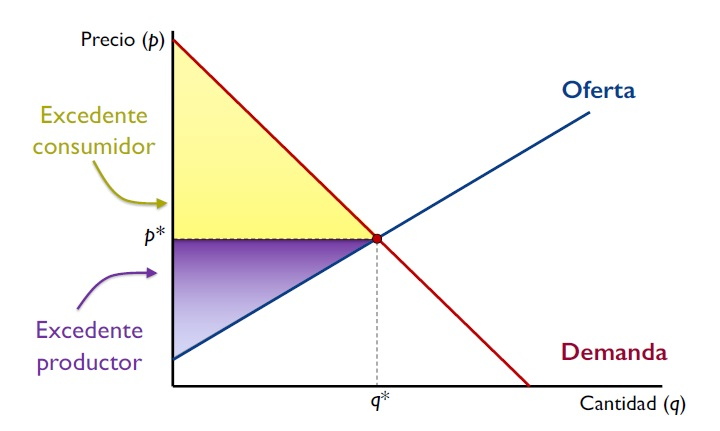
\includegraphics[scale=0.55]{../Figures/Tema_07.23_equilibrioyexcedente.jpg}
\end{center}
\end{frame}

\begin{frame}
\frametitle{¿Por qué es eficiente?}
\begin{itemize}
    \item Los participantes son tomadores de precios
    \begin{itemize}
        \item No hay poder de mercado.
        \item La competencia impide a los vendedores aumentar el precio, y a los compradores bajarlo.
    \end{itemize}
    \item No hay barreras de entrada
    \item Los contratos son completos
        \begin{itemize}
        \item Los detalles del intercambio pueden ser definidos en forma clara, y estos contratos se pueden hacer cumplir.
        \end{itemize}
    \item No hay externalidades
        \begin{itemize}
        \item La transacción sólo afecta a los compradores y vendedores
        \end{itemize}
\end{itemize}
\end{frame}

\begin{frame}{¿Por qué es eficiente?}
    \begin{center}
        
\includegraphics[scale=0.55]{../Figures/DNU_Milei.png}
    \end{center}
\end{frame}

\begin{frame}
\frametitle{Resumen...}
\small
\begin{center}
    \begin{tabular}{c|c}
    \hline
    \hline
    Tomadores de precios & Fijadores de precio \\
    Competencia Perfecta & Monopolio
    \\
    \hline
    \hline
    Puede ser   &  \\ 
    Pareto eficiente & 
    \\
    \hline
    No hay rentas &  \\
    económicas en &  \\
    el largo plazo & 
    \\
    \hline
    Poca gasto en su &  \\ publicidad & 
    \\
    \hline
    Pocos incentivos para &   \\ 
    la innovación porque &  \\
    porque otras van a copiar & 
\end{tabular}
\end{center}
\end{frame}


\end{document}
